\UseRawInputEncoding
\documentclass[11pt,a4paper]{article}
\usepackage[margin=0.7in]{geometry}
\usepackage{booktabs}
\usepackage[hidelinks]{hyperref}
\usepackage{float}
\usepackage{amsmath}
\usepackage{graphicx}

\title{\textbf{Information Retrieval and Extraction --- Assignment 2:\\Learning from Click-Logs on EB-NeRD and MIND}}
\author{Piyush Kumar Agarwal(2025201082) \\KSPSVLN Siddhardha Kumar Kavuri(2025201061) \\ [0.4em]
\normalsize Code: \protect\url{https://github.com/piyukr2/IRE_assignment_1/tree/assignment-2}}
\date{}

\begin{document}
\maketitle

\section*{1. What we built}

A two-stage retrieve-then-rank pipeline on both datasets. Stage one is
Assignment 1's candidate generator (BM25 and multilingual sentence embeddings).
Stage two is a re-ranker trained on click-log features. Everything is split
\emph{temporally}: the re-ranker is fitted on the train period, stopped early on
the validation period, and reported on the test period (2{,}000 test impressions
per dataset, the same set for every model). We evaluate on \texttt{mind\_small}
and \texttt{ebnerd\_small}.

\textbf{What is re-ranked.} Each impression's own candidate list (the serving path in Section 5 uses an ANN top-200, $K=200$).

\textbf{Features} (nine, shared by both hand-crafted re-rankers):
\begin{itemize}\itemsep0pt
\item \emph{Retrieval:} \texttt{bm25\_score}, \texttt{semantic\_score}.
\item \emph{Click history:} \texttt{n\_clicks\_in\_history}, and
  \texttt{recency\_weighted\_click\_count} (exponential decay, closed form
  $(1-d^{n})/(1-d)$).
\item \emph{Article:} \texttt{popularity\_train} (clicks in the training split
  only), \texttt{category\_match} with the user's history, \texttt{has\_published\_time}.
\item \emph{Session (EB-NeRD only):} \texttt{session\_click\_count},
  \texttt{position\_in\_session}. MIND has no sessions, so these are absent there
  rather than replaced by a proxy.
\end{itemize}
Freshness is not a model input (MIND ships no publication time). Dwell time is post-click, so it appears only in the ablation of Section 7.
Behaviour window: a user's history for an impression contains only clicks strictly before its timestamp.

\textbf{Re-rankers.} (A) LightGBM \texttt{lambdarank}; (B) a small MLP, pointwise, on the same nine features; (C) an NRMS-style neural ranker over the click history (Section 3). All trainers are seeded and deterministic.

\section*{2. Re-ranker results: before and after (Q2)}

\begin{table}[H]
\centering\footnotesize\setlength{\tabcolsep}{4pt}
\begin{tabular}{llrrrrl}
\toprule
\textbf{Dataset} & \textbf{Model} & \textbf{AUC} & \textbf{MRR} & \textbf{nDCG@5} & \textbf{nDCG@10} & \textbf{$\Delta$ nDCG@10 [95\% CI]} \\
\midrule
\texttt{ebnerd\_small} & Retrieval only & 0.5505 & 0.3475 & 0.3867 & 0.4676 &  \\
 & GBDT (LightGBM) & 0.4716 & 0.2770 & 0.3098 & 0.4045 & $-$0.0632 [$-$0.0745, $-$0.0511] \\
 & MLP & 0.5370 & 0.3285 & 0.3704 & 0.4536 & $-$0.0140 [$-$0.0230, $-$0.0050] \\
\midrule
\texttt{mind\_small} & Retrieval only & 0.5985 & 0.3187 & 0.3039 & 0.3597 &  \\
 & GBDT (LightGBM) & 0.6125 & 0.3390 & 0.3184 & 0.3771 & +0.0174 [+0.0062, +0.0286] \\
 & MLP & 0.6169 & 0.3446 & 0.3225 & 0.3800 & +0.0203 [+0.0096, +0.0317] \\
\bottomrule
\end{tabular}
\caption{Test split, 2{,}000 impressions. $\Delta$ is the paired-bootstrap difference from ``Retrieval only''; ``n.s.'' marks an interval that includes zero; unmarked intervals exclude zero.}
\end{table}

\textbf{Observation.} Both re-rankers beat retrieval-only on MIND (intervals exclude zero) and fall below it on EB-NeRD.

\section*{3. Baseline reproduced, then improved (Q3)}

\textbf{Reproduction.} NRMS scores the dot product of a news vector and a user vector. We implement the click-level half as published (multi-head self-attention over past clicks, then additive attention) and replace the word-level half with the pinned 384-dimensional sentence embeddings from Assignment 1. Training is listwise (softmax over one clicked and four sampled non-clicked candidates). Hyperparameters are our own declared choices. The baseline is the retrieval-only \texttt{semantic\_score}.

\textbf{The one principled change: category-aware encoding.} A learned category embedding is concatenated to every article vector; the two NRMS models differ only by it (a test asserts this).

\begin{table}[H]
\centering\footnotesize\setlength{\tabcolsep}{4pt}
\begin{tabular}{llrrrrl}
\toprule
\textbf{Dataset} & \textbf{Model} & \textbf{AUC} & \textbf{MRR} & \textbf{nDCG@5} & \textbf{nDCG@10} & \textbf{$\Delta$ nDCG@10 [95\% CI]} \\
\midrule
\texttt{ebnerd\_small} & Retrieval only & 0.5505 & 0.3475 & 0.3867 & 0.4676 &  \\
 & NRMS reproduction & 0.5631 & 0.3556 & 0.3968 & 0.4736 & +0.0060 [$-$0.0070, +0.0205] n.s. \\
 & NRMS + category & 0.5895 & 0.3728 & 0.4193 & 0.4897 & +0.0221 [+0.0081, +0.0362] \\
\midrule
\texttt{mind\_small} & Retrieval only & 0.5985 & 0.3187 & 0.3039 & 0.3597 &  \\
 & NRMS reproduction & 0.6008 & 0.3200 & 0.3027 & 0.3645 & +0.0048 [$-$0.0093, +0.0187] n.s. \\
 & NRMS + category & 0.6145 & 0.3240 & 0.2996 & 0.3675 & +0.0078 [$-$0.0061, +0.0206] n.s. \\
\bottomrule
\end{tabular}
\caption{Test split, 2{,}000 impressions. $\Delta$ is the paired-bootstrap difference from retrieval only (1{,}000 resamples over impressions); ``n.s.'' marks an interval that includes zero.}
\end{table}

\textbf{Ablation.} Because the two NRMS models differ by exactly one component,
their difference isolates it.

\begin{table}[H]
\centering\small
\begin{tabular}{lrcc}
\toprule
\textbf{Dataset} & \textbf{nDCG@10: category-aware $-$ reproduction} & \textbf{95\% CI} & \textbf{Excludes zero?} \\
\midrule
\texttt{ebnerd\_small} & +0.0161 & [+0.0065, +0.0262] & yes \\
\texttt{mind\_small} & +0.0030 & [$-$0.0054, +0.0113] & no \\
\bottomrule
\end{tabular}
\end{table}

The gain is claimed on EB-NeRD only; on MIND the interval includes zero.

\section*{4. Extended evaluation of the full pipeline (Q5)}

All seven metrics with paired-bootstrap 95\% intervals, computed by Assignment
1's harness unchanged, for retrieval-only and for retrieval plus the
category-aware NRMS re-ranker.

\begin{table}[H]
\centering\scriptsize
\setlength{\tabcolsep}{3pt}
\begin{tabular}{lcccc}
\toprule
 & \multicolumn{2}{c}{\texttt{ebnerd\_small}} & \multicolumn{2}{c}{\texttt{mind\_small}} \\
\cmidrule(lr){2-3}\cmidrule(lr){4-5}
\textbf{Metric} & retrieval only & + NRMS category & retrieval only & + NRMS category \\
\midrule
AUC & 0.5505 [0.5357, 0.5646] & 0.5895 [0.5751, 0.6013] & 0.5985 [0.5849, 0.6113] & 0.6145 [0.6023, 0.6271] \\
MRR & 0.3475 [0.3344, 0.3604] & 0.3728 [0.3601, 0.3855] & 0.3187 [0.3050, 0.3332] & 0.3240 [0.3103, 0.3379] \\
nDCG@5 & 0.3867 [0.3715, 0.4009] & 0.4193 [0.4041, 0.4331] & 0.3039 [0.2883, 0.3194] & 0.2996 [0.2845, 0.3139] \\
nDCG@10 & 0.4676 [0.4554, 0.4800] & 0.4897 [0.4776, 0.5016] & 0.3597 [0.3455, 0.3743] & 0.3675 [0.3540, 0.3816] \\
Diversity & 0.1739 [0.1733, 0.1745] & 0.1782 [0.1777, 0.1787] & 0.2238 [0.2230, 0.2247] & 0.2376 [0.2371, 0.2381] \\
Novelty & 17.2840 [17.2503, 17.3167] & 17.3224 [17.2882, 17.3546] & 17.2391 [17.2038, 17.2730] & 17.6126 [17.5900, 17.6339] \\
Coverage & 0.0749 [0.0650, 0.0680] & 0.0745 [0.0644, 0.0675] & 0.0142 [0.0115, 0.0124] & 0.0146 [0.0116, 0.0125] \\
\bottomrule
\end{tabular}
\caption{Coverage is the size of a union rather than an average, so its point estimate lies outside its bootstrap interval; the interval describes sampling variability only.}
\end{table}

\textbf{Slices.} Cold-start vs warm (whether the user has any prior click) and
head vs tail (an impression is ``head'' if a clicked article is among the
popular ones, popularity measured on the test period; an analysis label, never a
model input). nDCG@10 with 95\% intervals:

\begin{table}[H]
\centering\footnotesize
\begin{tabular}{llrcc}
\toprule
\textbf{Dataset} & \textbf{Slice} & \textbf{n} & \textbf{Retrieval only} & \textbf{+ NRMS category} \\
\midrule
\texttt{ebnerd\_small} & cold start & 0 & \multicolumn{2}{c}{no impressions} \\
 & warm & 2,000 & 0.4676 [0.4554, 0.4800] & 0.4897 [0.4776, 0.5016] \\
 & head & 1,019 & 0.4525 [0.4360, 0.4693] & 0.4768 [0.4589, 0.4951] \\
 & tail & 981 & 0.4833 [0.4658, 0.4990] & 0.5032 [0.4863, 0.5202] \\
\midrule
\texttt{mind\_small} & cold start & 62 & 0.3201 [0.2344, 0.4137] & 0.3908 [0.3183, 0.4720] \\
 & warm & 1,938 & 0.3610 [0.3461, 0.3758] & 0.3668 [0.3532, 0.3814] \\
 & head & 1,194 & 0.4180 [0.3995, 0.4366] & 0.4537 [0.4355, 0.4709] \\
 & tail & 806 & 0.2734 [0.2499, 0.2973] & 0.2398 [0.2196, 0.2601] \\
\bottomrule
\end{tabular}
\end{table}

\textbf{Observation.} Cold-start gains most on MIND, but $n=62$ is too small for the interval to be trusted; EB-NeRD has no cold-start users in its sample.

\section*{5. Serving and scale (Q4)}

Measured at batch size one on CPU, 50 warm-up requests discarded and 1{,}000
measured. One request: pool a user vector, ANN top-200 over the corpus, BM25 over
those candidates, assemble the feature row, score, tie-break.

\begin{table}[H]
\centering\small
\begin{tabular}{lrr}
\toprule
 & \texttt{ebnerd\_small} & \texttt{mind\_small} \\
\midrule
p50 / p95 / \textbf{p99} latency (ms) & 4.13 / 5.36 / \textbf{6.15} & 5.61 / 6.26 / \textbf{6.68} \\
\quad ANN search p99 (ms) & 2.64 & 3.87 \\
\quad feature build p99 (ms) & 1.41 & 1.50 \\
\quad re-ranker forward pass p99 (ms) & 0.06 & 0.07 \\
ANN index on disk (MB) & 37.5 & 118.0 \\
Embedding matrix in RAM (MB) & 31.9 & 100.2 \\
Feature store on disk (MB) & 111.8 & 95.1 \\
Feature store in RAM (MB) & 724.6 & 366.8 \\
Core-seconds per 1{,}000 queries & 4.26 & 5.53 \\
Sustainable QPS on 4 cores (p99 $<$ 100\,ms) & 940 & 723 \\
\bottomrule
\end{tabular}
\caption{One benchmark run on this machine; latencies vary between runs. Cost is given as core-seconds because we have no dated, citable instance price, and an invented price would be a number that traces to nothing.}
\end{table}

The p99 target of 100\,ms is met on both datasets; ANN search is the slowest stage at p99.

\section*{6. Where it breaks at $10\times$}

\begin{enumerate}\itemsep0pt
\item \textbf{In-RAM inverted index and feature store} grow linearly with the corpus, so memory breaks first.
\item \textbf{Embedding matrix} (about 100\,MB on MIND, about 1\,GB at $10\times$) competes with the encoder for 4\,GB of VRAM; scoring against a memory-mapped matrix is the fix.
\item \textbf{Per-candidate Python work} in the feature build scales with candidate count; a per-impression loop already broke before the model did in Assignment 1 (37 hours vs 14 minutes once vectorised).
\item \textbf{Train/serve skew:} \texttt{popularity\_train} is non-zero for only 5.6\% of MIND and 8.2\% of EB-NeRD submission candidates (samples of 20{,}000 MIND lines and 50{,}000 EB-NeRD rows), and the EB-NeRD test file has no clicks, so \texttt{session\_click\_count} has no source. The NRMS ranker uses only embeddings and a category label, so it is the model we submit.
\end{enumerate}

\section*{7. Anti-gaming (Q9)}

\textbf{Metrics with and without features unavailable at serving time.} We add the dataset-wide aggregates \texttt{total\_inviews}, \texttt{total\_pageviews}, \texttt{total\_read\_time} to the MLP re-ranker in a labelled ablation (EB-NeRD; MIND ships none of them).

\begin{table}[H]
\centering\small
\begin{tabular}{lrrrr}
\toprule
\textbf{EB-NeRD, MLP re-ranker} & \textbf{AUC} & \textbf{MRR} & \textbf{nDCG@5} & \textbf{nDCG@10} \\
\midrule
Serving-available features only (headline) & 0.5369 & 0.3277 & 0.3675 & 0.4533 \\
+ \texttt{total\_*} aggregates (ablation) & 0.5918 & 0.3679 & 0.4147 & 0.4897 \\
\bottomrule
\end{tabular}
\caption{Adding the unavailable features changes nDCG@10 by +0.0364 [+0.0256, +0.0469] (95\% CI). }
\end{table}

\textbf{No future-click leakage.} Tests check per-feature values, per-row split membership and the neural model's history tensor; canary tests (including a click at exactly the impression time) show they can fail.

\section*{8. Codabench leaderboards (Q5, Q7)}

Both submissions use the category-aware NRMS ranker over the complete large test
sets (2{,}370{,}727 MIND impressions; 13{,}536{,}710 EB-NeRD rows).

\begin{table}[H]
\centering\small
\begin{tabular}{llrrrr}
\toprule
\textbf{Competition} & \textbf{Submission} & \textbf{AUC} & \textbf{MRR} & \textbf{nDCG@5} & \textbf{nDCG@10} \\
\midrule
MIND    & A2: NRMS + category          & 0.6290 & 0.2905 & 0.3122 & 0.3700 \\
        & A1: BM25 + semantic hybrid   & 0.6114 & 0.2969 & 0.3179 & 0.3732 \\
\midrule
EB-NeRD & A2: NRMS + category          & \multicolumn{4}{c}{first upload failed; resubmission running, no score yet} \\
        & A1: semantic retrieval       & 0.5508 & 0.3510 & 0.3916 & 0.4679 \\
\bottomrule
\end{tabular}
\caption{Scores returned by the Codabench scorers. Grading is not on rank; Assignment 1 rows are shown for reference.}
\end{table}

\textbf{MIND.} NRMS is ahead of the Assignment 1 hybrid on AUC and slightly behind on MRR, nDCG@5 and nDCG@10.

\textbf{EB-NeRD.} The first NRMS submission (\#931721) failed at Codabench and has no score (all status fields null). We verified the file: all 13{,}536{,}710 rows have the right number of ranks, in order, as a valid permutation, in a single \texttt{predictions.txt} that passes \texttt{unzip -t}. The same file was resubmitted (\#935074) and had not finished when this report was written, so the NRMS result for EB-NeRD is reported offline only (Sections 3 and 4).

\begin{figure}[H]
\centering
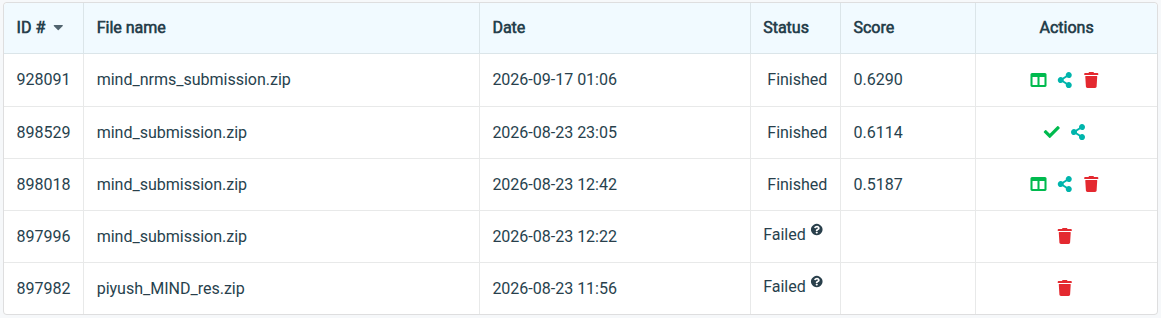
\includegraphics[width=0.85\linewidth]{MIND_A1_C2.png}
\caption{MIND competition, ``My submissions'': the NRMS submission (top row) scored 0.6290.}
\end{figure}

\begin{figure}[H]
\centering
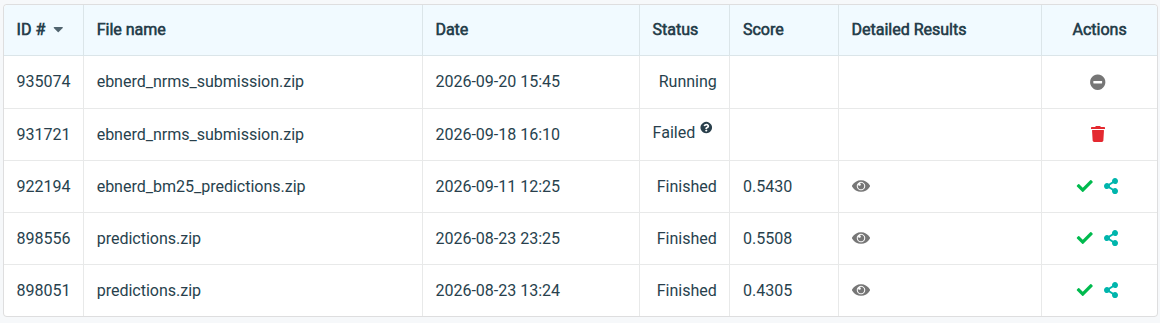
\includegraphics[width=0.85\linewidth]{EbNERD_A1_C2.png}
\caption{EB-NeRD competition, ``My submissions'': the first NRMS submission (\#931721) shows \emph{Failed}; the resubmission (\#935074, top row) was still \emph{Running} when this report was written.}
\end{figure}

\section*{Reproducing}

\begin{verbatim}
make setup && make test            # no dataset and no GPU required
make clean-derived && make all     # every Assignment 1 number
make a2-all                        # the A2 stages (these train, so GPU-only)
make submit-nrms                   # the two Codabench prediction files
\end{verbatim}
The AI usage log is in \texttt{ai\_usage/}.

\end{document}
